\documentclass{standalone}
\usepackage{tikz}
\usetikzlibrary{patterns, positioning}


\begin{document}
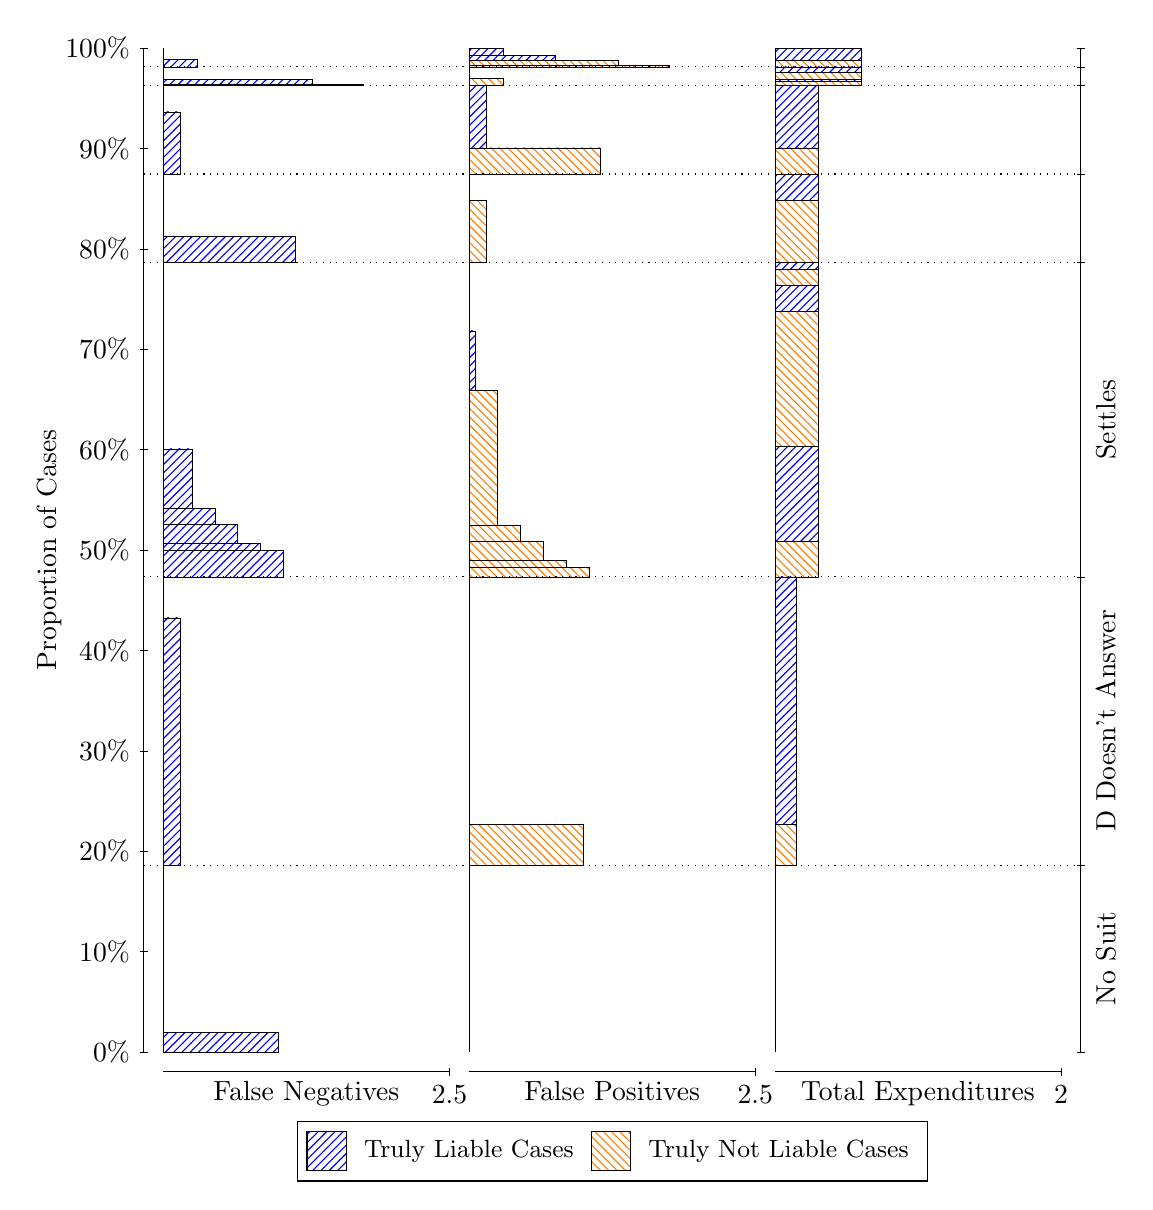
\begin{tikzpicture}
\draw[black, very thin] (1.5,1.75) -- (1.5,14.5);
\node[rotate=90, text=black, anchor=center] at (0.3, 8.125) {Proportion of Cases};
\draw[black, very thin] (1.45,1.75) -- (1.55,1.75);
\node[text=black, anchor=east] at (1.45, 1.75) {0\%};
\draw[black, very thin] (1.45,3.025) -- (1.55,3.025);
\node[text=black, anchor=east] at (1.45, 3.025) {10\%};
\draw[black, very thin] (1.45,4.3) -- (1.55,4.3);
\node[text=black, anchor=east] at (1.45, 4.3) {20\%};
\draw[black, very thin] (1.45,5.575) -- (1.55,5.575);
\node[text=black, anchor=east] at (1.45, 5.575) {30\%};
\draw[black, very thin] (1.45,6.85) -- (1.55,6.85);
\node[text=black, anchor=east] at (1.45, 6.85) {40\%};
\draw[black, very thin] (1.45,8.125) -- (1.55,8.125);
\node[text=black, anchor=east] at (1.45, 8.125) {50\%};
\draw[black, very thin] (1.45,9.4) -- (1.55,9.4);
\node[text=black, anchor=east] at (1.45, 9.4) {60\%};
\draw[black, very thin] (1.45,10.675) -- (1.55,10.675);
\node[text=black, anchor=east] at (1.45, 10.675) {70\%};
\draw[black, very thin] (1.45,11.95) -- (1.55,11.95);
\node[text=black, anchor=east] at (1.45, 11.95) {80\%};
\draw[black, very thin] (1.45,13.225) -- (1.55,13.225);
\node[text=black, anchor=east] at (1.45, 13.225) {90\%};
\draw[black, very thin] (1.45,14.5) -- (1.55,14.5);
\node[text=black, anchor=east] at (1.45, 14.5) {100\%};

\draw[black, very thin] (13.4,1.75) -- (13.4,14.5);
\draw[black, very thin] (13.35,1.75) -- (13.45,1.75);
\node[anchor=west] at (13.35, 1.75) {};
\draw[black, very thin] (13.35,4.1224) -- (13.45,4.1224);
\node[anchor=west] at (13.35, 4.1224) {};
\draw[black, very thin] (13.35,7.7848) -- (13.45,7.7848);
\node[anchor=west] at (13.35, 7.7848) {};
\draw[black, very thin] (13.35,11.777) -- (13.45,11.777);
\node[anchor=west] at (13.35, 11.777) {};
\draw[black, very thin] (13.35,12.9) -- (13.45,12.9);
\node[anchor=west] at (13.35, 12.9) {};
\draw[black, very thin] (13.35,14.022) -- (13.45,14.022);
\node[anchor=west] at (13.35, 14.022) {};
\draw[black, very thin] (13.35,14.261) -- (13.45,14.261);
\node[anchor=west] at (13.35, 14.261) {};
\draw[black, very thin] (13.35,14.5) -- (13.45,14.5);
\node[anchor=west] at (13.35, 14.5) {};

\draw[black, very thin, pattern color=blue, pattern=north east lines] (1.75,1.75) rectangle (3.2033,1.9996);
\draw[black, very thin, pattern color=orange, pattern=north west lines] (1.75,1.9996) rectangle (1.75,4.1224);
\draw[black, very thin, pattern color=blue, pattern=north east lines] (1.75,4.1224) rectangle (1.968,7.2635);
\draw[black, very thin, pattern color=orange, pattern=north west lines] (1.75,7.2635) rectangle (1.75,7.7848);
\draw[black, very thin, pattern color=blue, pattern=north east lines] (1.75,7.7848) rectangle (3.276,8.1159);
\draw[black, very thin, pattern color=blue, pattern=north east lines] (1.75,8.1159) rectangle (2.9853,8.2081);
\draw[black, very thin, pattern color=blue, pattern=north east lines] (1.75,8.2081) rectangle (2.6947,8.4494);
\draw[black, very thin, pattern color=blue, pattern=north east lines] (1.75,8.4494) rectangle (2.404,8.6531);
\draw[black, very thin, pattern color=blue, pattern=north east lines] (1.75,8.6531) rectangle (2.1133,9.4078);
\draw[black, very thin, pattern color=orange, pattern=north west lines] (1.75,9.4078) rectangle (1.75,11.777);
\draw[black, very thin, pattern color=blue, pattern=north east lines] (1.75,11.777) rectangle (3.4213,12.11);
\draw[black, very thin, pattern color=orange, pattern=north west lines] (1.75,12.11) rectangle (1.75,12.9);
\draw[black, very thin, pattern color=blue, pattern=north east lines] (1.75,12.9) rectangle (1.968,13.689);
\draw[black, very thin, pattern color=orange, pattern=north west lines] (1.75,13.689) rectangle (1.75,14.022);
\draw[black, very thin, pattern color=blue, pattern=north east lines] (1.75,14.022) rectangle (4.2933,14.041);
\draw[black, very thin, pattern color=blue, pattern=north east lines] (1.75,14.041) rectangle (3.6393,14.106);
\draw[black, very thin, pattern color=orange, pattern=north west lines] (1.75,14.106) rectangle (1.75,14.261);
\draw[black, very thin, pattern color=blue, pattern=north east lines] (1.75,14.261) rectangle (2.186,14.356);
\draw[black, very thin, pattern color=orange, pattern=north west lines] (1.75,14.356) rectangle (1.75,14.44);
\draw[black, very thin, pattern color=blue, pattern=north east lines] (1.75,14.44) rectangle (1.75,14.5);
\draw[black, very thin, pattern color=orange, pattern=north west lines] (5.6333,1.75) rectangle (5.6333,3.8728);
\draw[black, very thin, pattern color=blue, pattern=north east lines] (5.6333,3.8728) rectangle (5.6333,4.1224);
\draw[black, very thin, pattern color=orange, pattern=north west lines] (5.6333,4.1224) rectangle (7.0867,4.6437);
\draw[black, very thin, pattern color=blue, pattern=north east lines] (5.6333,4.6437) rectangle (5.6333,7.7848);
\draw[black, very thin, pattern color=orange, pattern=north west lines] (5.6333,7.7848) rectangle (7.1593,7.9042);
\draw[black, very thin, pattern color=orange, pattern=north west lines] (5.6333,7.9042) rectangle (6.8687,7.9965);
\draw[black, very thin, pattern color=orange, pattern=north west lines] (5.6333,7.9965) rectangle (6.578,8.2378);
\draw[black, very thin, pattern color=orange, pattern=north west lines] (5.6333,8.2378) rectangle (6.2873,8.4414);
\draw[black, very thin, pattern color=orange, pattern=north west lines] (5.6333,8.4414) rectangle (5.9967,10.154);
\draw[black, very thin, pattern color=blue, pattern=north east lines] (5.6333,10.154) rectangle (5.706,10.909);
\draw[black, very thin, pattern color=blue, pattern=north east lines] (5.6333,10.909) rectangle (5.6333,11.777);
\draw[black, very thin, pattern color=orange, pattern=north west lines] (5.6333,11.777) rectangle (5.8513,12.567);
\draw[black, very thin, pattern color=blue, pattern=north east lines] (5.6333,12.567) rectangle (5.6333,12.9);
\draw[black, very thin, pattern color=orange, pattern=north west lines] (5.6333,12.9) rectangle (7.3047,13.232);
\draw[black, very thin, pattern color=blue, pattern=north east lines] (5.6333,13.232) rectangle (5.8513,14.022);
\draw[black, very thin, pattern color=orange, pattern=north west lines] (5.6333,14.022) rectangle (6.0693,14.117);
\draw[black, very thin, pattern color=orange, pattern=north west lines] (5.6333,14.117) rectangle (5.6333,14.176);
\draw[black, very thin, pattern color=blue, pattern=north east lines] (5.6333,14.176) rectangle (5.6333,14.261);
\draw[black, very thin, pattern color=orange, pattern=north west lines] (5.6333,14.261) rectangle (8.1767,14.28);
\draw[black, very thin, pattern color=orange, pattern=north west lines] (5.6333,14.28) rectangle (7.5227,14.345);
\draw[black, very thin, pattern color=blue, pattern=north east lines] (5.6333,14.345) rectangle (6.7233,14.405);
\draw[black, very thin, pattern color=blue, pattern=north east lines] (5.6333,14.405) rectangle (6.0693,14.5);
\draw[black, very thin, pattern color=orange, pattern=north west lines] (9.5167,1.75) rectangle (9.5167,3.8728);
\draw[black, very thin, pattern color=blue, pattern=north east lines] (9.5167,3.8728) rectangle (9.5167,4.1224);
\draw[black, very thin, pattern color=orange, pattern=north west lines] (9.5167,4.1224) rectangle (9.7892,4.6437);
\draw[black, very thin, pattern color=blue, pattern=north east lines] (9.5167,4.6437) rectangle (9.7892,7.7848);
\draw[black, very thin, pattern color=orange, pattern=north west lines] (9.5167,7.7848) rectangle (10.062,8.2378);
\draw[black, very thin, pattern color=blue, pattern=north east lines] (9.5167,8.2378) rectangle (10.062,9.4374);
\draw[black, very thin, pattern color=orange, pattern=north west lines] (9.5167,9.4374) rectangle (10.062,11.151);
\draw[black, very thin, pattern color=blue, pattern=north east lines] (9.5167,11.151) rectangle (10.062,11.482);
\draw[black, very thin, pattern color=orange, pattern=north west lines] (9.5167,11.482) rectangle (10.062,11.685);
\draw[black, very thin, pattern color=blue, pattern=north east lines] (9.5167,11.685) rectangle (10.062,11.777);
\draw[black, very thin, pattern color=orange, pattern=north west lines] (9.5167,11.777) rectangle (10.062,12.567);
\draw[black, very thin, pattern color=blue, pattern=north east lines] (9.5167,12.567) rectangle (10.062,12.9);
\draw[black, very thin, pattern color=orange, pattern=north west lines] (9.5167,12.9) rectangle (10.062,13.232);
\draw[black, very thin, pattern color=blue, pattern=north east lines] (9.5167,13.232) rectangle (10.062,14.022);
\draw[black, very thin, pattern color=orange, pattern=north west lines] (9.5167,14.022) rectangle (10.607,14.081);
\draw[black, very thin, pattern color=blue, pattern=north east lines] (9.5167,14.081) rectangle (10.607,14.1);
\draw[black, very thin, pattern color=orange, pattern=north west lines] (9.5167,14.1) rectangle (10.607,14.195);
\draw[black, very thin, pattern color=blue, pattern=north east lines] (9.5167,14.195) rectangle (10.607,14.261);
\draw[black, very thin, pattern color=orange, pattern=north west lines] (9.5167,14.261) rectangle (10.607,14.345);
\draw[black, very thin, pattern color=blue, pattern=north east lines] (9.5167,14.345) rectangle (10.607,14.5);
\draw[black, dotted] (1.5,4.1224) -- (13.4,4.1224);
\draw[black, dotted] (1.5,7.7848) -- (13.4,7.7848);
\draw[black, dotted] (1.5,11.777) -- (13.4,11.777);
\draw[black, dotted] (1.5,12.9) -- (13.4,12.9);
\draw[black, dotted] (1.5,14.022) -- (13.4,14.022);
\draw[black, dotted] (1.5,14.261) -- (13.4,14.261);
\draw[black, very thin] (1.75,1.5) -- (5.3833,1.5);
\node[text=black, anchor=north] at (3.5667, 1.5) {False Negatives};
\draw[black, very thin] (5.3833,1.45) -- (5.3833,1.55);
\node[text=black, anchor=north] at (5.3833, 1.45) {2.5};

\draw[black, very thin] (5.6333,1.5) -- (9.2667,1.5);
\node[text=black, anchor=north] at (7.45, 1.5) {False Positives};
\draw[black, very thin] (9.2667,1.45) -- (9.2667,1.55);
\node[text=black, anchor=north] at (9.2667, 1.45) {2.5};

\draw[black, very thin] (9.5167,1.5) -- (13.15,1.5);
\node[text=black, anchor=north] at (11.333, 1.5) {Total Expenditures};
\draw[black, very thin] (13.15,1.45) -- (13.15,1.55);
\node[text=black, anchor=north] at (13.15, 1.45) {2};

\node[text=black, centered, rotate=90] at (13.72, 2.9362) {No Suit};
\node[text=black, centered, rotate=90] at (13.72, 5.9536) {D Doesn't Answer};
\node[text=black, centered, rotate=90] at (13.72, 9.7811) {Settles};





\draw (7.449999999999999,1.5) node[draw=none] (baseCoordinate) {};
\begin{scope}[align=center]
        \matrix[scale=0.5, draw=black, below=0.5cm of baseCoordinate, nodes={draw}, column sep=0.1cm]{
            \node[rectangle, draw, minimum width=0.5cm, minimum height=0.5cm, pattern color=blue, pattern=north east lines] {}; &
            \node[draw=none, font=\small, text=black] (B) {Truly Liable Cases}; &
            \node[rectangle, draw, minimum width=0.5cm, minimum height=0.5cm, pattern color=orange, pattern=north west lines] {}; &
            \node[draw=none, font=\small, text=black] (B) {Truly Not Liable Cases}; \\
            };
\end{scope}

\end{tikzpicture}
\end{document}